% Section content template for individual Educative lessons
% This file contains the actual content for a specific section
% Generated from Educative API section content

% Section: Requirements of a Distributed Search System's Design
% Section ID: 5706146547761152
% Section Slug: requirements-of-a-distributed-search-systems-design
% Generated: 2025-12-07T21:51:24.526962

\subsection{Requirements}\label{UdKA3rm8sglvurUtytsNx}
\\
Let's understand the functional and non-functional requirements of a distributed search system.

\subsubsection{Functional requirements}\label{3wjG1DWsecTOVRIS8V4mH}
\\
The following is a functional requirement of a distributed search system:

\begin{itemize}
\item
\protect\phantomsection\label{TTcHsUAPRavIZL0tTfnr3}
\textbf{Search}: Users should get relevant content based on their search queries.
\end{itemize}

\begin{figure}[htbp]
 \centering
 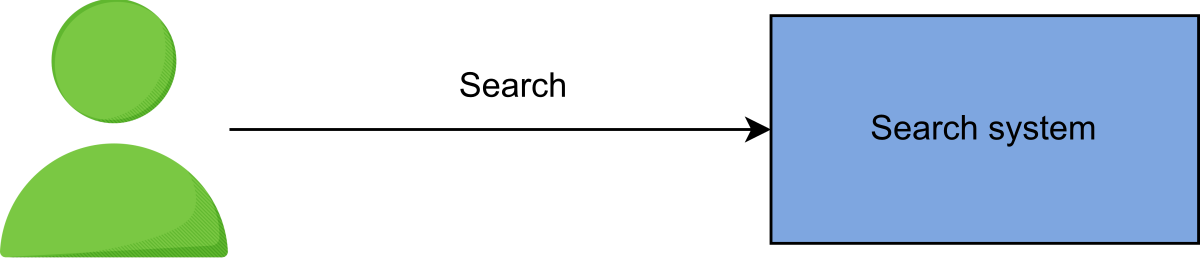
\includegraphics[width=0.5\textwidth]{Images/chapter_21/section_5706146547761152/5603209773449216.png}
 \caption{The functional requirement of a distributed search system}
\end{figure}

\subsubsection{Non-functional requirements}\label{WyNwatnmMweiKkDkbXbBr}
\\
Here are the non-functional requirements of a distributed search system:

\begin{itemize}
\item
\protect\phantomsection\label{GmHDEUY2c6Y5VqG9J-_3f}
\textbf{Availability}: The system should be highly available to the users.
\item
\protect\phantomsection\label{xH6AawJhmfUSHOuZYr4jW}
\textbf{Scalability}: The system should have the ability to scale with the increasing amount of data. In other words, it should be able to index a large amount of data.
\item
\protect\phantomsection\label{GSv_xkOBHGUMlqMw7bGsc}
\textbf{Fast search on big data}: The user should get the results quickly, no matter how much content they are searching.
\item
\protect\phantomsection\label{erO9Zr53PpCzxysDcJ-aP}
\textbf{Reduced cost}: The overall cost of building a search system should be less.
\end{itemize}

\begin{figure}[htbp]
 \centering
 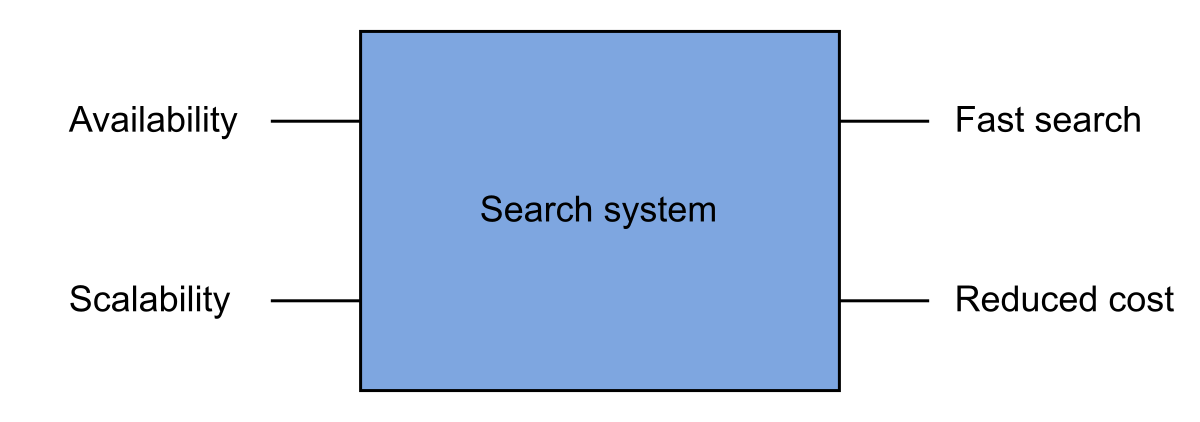
\includegraphics[width=0.3\textwidth]{Images/chapter_21/section_5706146547761152/6666357261467648.png}
 \caption{The non-functional requirement of a distributed search system}
\end{figure}

\subsection{Resource estimation}\label{H5ZiE1pFkedVNiNneWuXQ}
\\
Let's estimate the total number of servers, storage, and bandwidth that is required by the distributed search system. We 'll calculate these numbers using an example of a YouTube search.

\subsubsection{Number of servers estimation}\label{p_Vvp4jYK5fLLqeA-tYrB}
\\
To estimate the number of servers, we need to know the number of daily active users of YouTube search feature. Let 's assume that we have 150 million daily active users of YouTube utilizing the search feature. Considering our assumption of using \href{https://www.educative.io/courses/grokking-the-system-design-interview/put-back-of-the-envelope-numbers-in-perspective}{daily active users as a proxy} for the number of requests per second to find the number of servers for peak load times, we get 150 million requests per second. Then
, we use the following formula to calculate the number of servers:

\[
\text{Servers needed at peak load} = \frac{\text{Number of requests/second}}{\text{RPS of server}}
\]

Using 64,000 as an estimated RPS of a server from the \href{https://www.educative.io/courses/grokking-the-system-design-interview/put-back-of-the-envelope-numbers-in-perspective}{Back-of-the-envelope Calculations} chapter, the required servers are estimated as follows:

\[
\text{Servers needed at peak load} = \frac{150 \ \text{million}}{64,000} = 2343.75 \approx 2350 \ \text{servers}
\]

\begin{figure}[htbp]
 \centering
 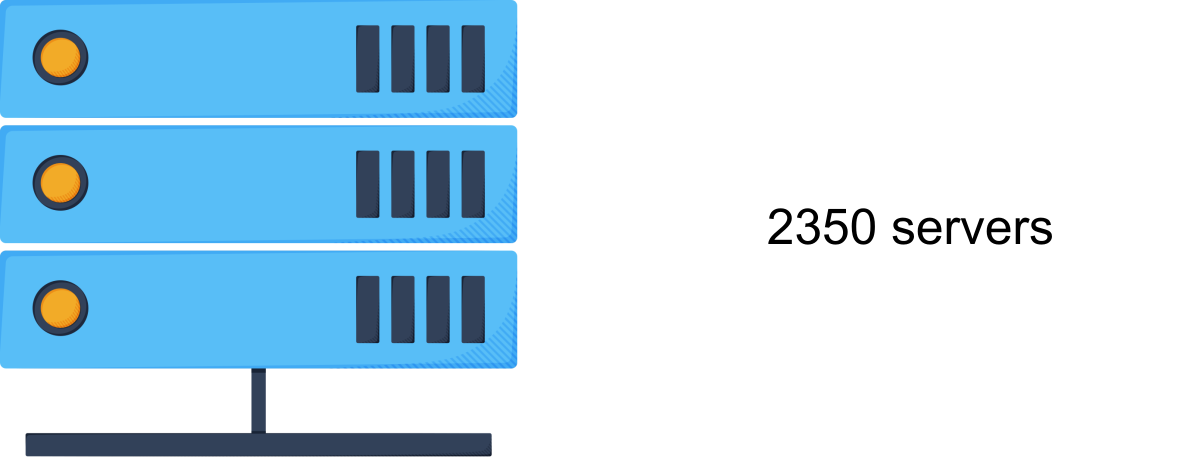
\includegraphics[width=0.25\textwidth]{Images/chapter_21/section_5706146547761152/5839232319225856.png}
 \caption{The number of servers required for the YouTube search service}
\end{figure}

\begin{quote}
\textbf{Note:} Concurrent requests significantly impact the number of required servers compared to requests spread over time.
\end{quote}
\subsubsection{Storage estimation}\label{bnW2wU1UrY9LsQ9D6a177}
\\
Each video's metadata is stored in a separate JSON document. Each document is uniquely identified by the video ID. This metadata contains the title of the video, its description, the channel name, and a transcript. We assume the following numbers for estimating the storage required to index one video:

\begin{itemize}
\item
\protect\phantomsection\label{tNNMR8YTnMCJXbOYvCLJi}
The size of a single JSON document is 200 KB.
\item
\protect\phantomsection\label{3BaN2t20TFwQkhHh9e3kG}
The number of unique terms or keys extracted from a single JSON document is 1,000.
\item
\protect\phantomsection\label{puRsVglFdhHfEsvX2cw9U}
The amount of storage space required to add one term into the index table is 100 Bytes.
\end{itemize}
\\
The following formula is used to compute the storage required to index one video:

\[
\text{Total}_{\text{storage/video}} = \text{Storage}_{\text{/doc}} + \left( \text{Terms}_{\text{/doc}} \times \text{Storage}_{\text{/term}} \right)
\]

In the table above, we calculate the storage required to index one video. We have already seen that the total storage required per video is 300 KB. Assuming that, on average, the number of videos uploaded per day on YouTube is 6,000, let's calculate the total storage required to index the videos uploaded per day. The following formula is used to compute the storage required to index the videos uploaded to YouTube in one day:

\[
\text{Total}_{\text{storage/day}} = \text{No. of videos}_{\text{/day}} \times \text{Total}_{\text{storage/video}}
\]

The total storage required to index 6,000 videos uploaded per day on YouTube is 1.8 GB. This storage requirement is just an estimation for YouTube. The storage need will increase if we provide a distributed search system as a service to multiple tenants.

\begin{figure}[htbp]
 \centering
 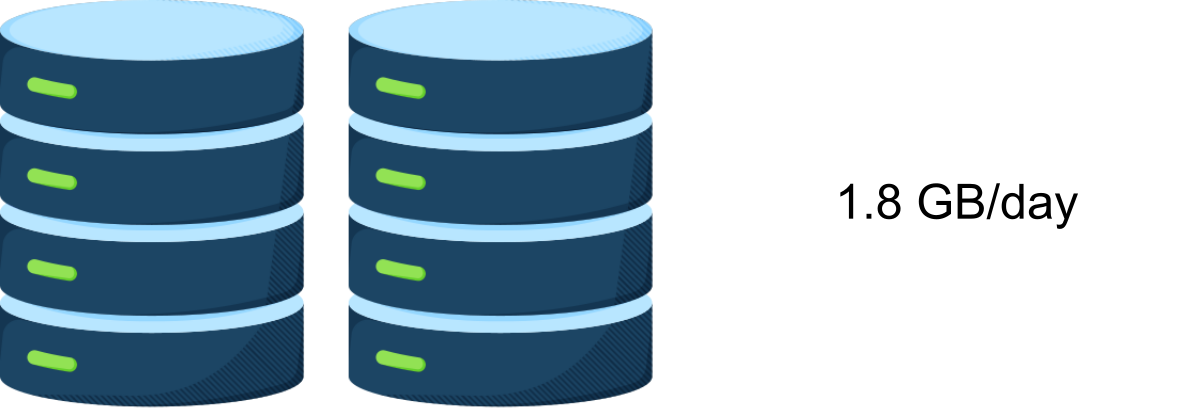
\includegraphics[width=0.25\textwidth]{Images/chapter_21/section_5706146547761152/6095133242425344.png}
 \caption{Summarizing the storage requirement of a distributed search system for videos uploaded to YouTube per day}
\end{figure}

\subsubsection{Bandwidth estimation}\label{mDdYMrj1AfhUx9iobhRwm}
\\
The data is transferred between the user and the server on each search request. We estimate the bandwidth required for the incoming traffic on the server and the outgoing traffic from the server. Here is the formula to calculate the required bandwidth:

\[
\text{Total}_{\text{bandwidth}} = \text{Total}_{\text{requests/second}} \times \text{Total}_{\text{query size}}
\]

\textbf{Incoming traffic}
\\
To estimate the incoming traffic bandwidth, we assume the following numbers:

\begin{itemize}
\item
\protect\phantomsection\label{qaFf8Xc8s5CR_FmdK9svv}
The number of search requests per day is 150 million.
\item
\protect\phantomsection\label{NoFFuD-X1CH754mOhu97k}
The search query size is 100 Bytes.
\end{itemize}

\textbf{Outgoing traffic}
\\
\textbf{Outgoing traffic} is the response that the server returns to the user on the search request. We assume that the number of suggested videos against a search query is 80, and one suggestion is of the size 50 Bytes. Suggestions consist of an ordered list of the video IDs.
\\
To estimate the outgoing traffic bandwidth, we assume the following numbers:

\begin{itemize}
\item
\protect\phantomsection\label{SoPPOxzodukA8IVrxKNEx}
The number of search requests per day is 150 million.
\item
\protect\phantomsection\label{xZbarV_SndCfgCC9LFb8w}
The response size is 4,000 Bytes.
\end{itemize}
\\
We can use the same formula to calculate the bandwidth required for the outgoing traffic.

\begin{figure}[htbp]
 \centering
 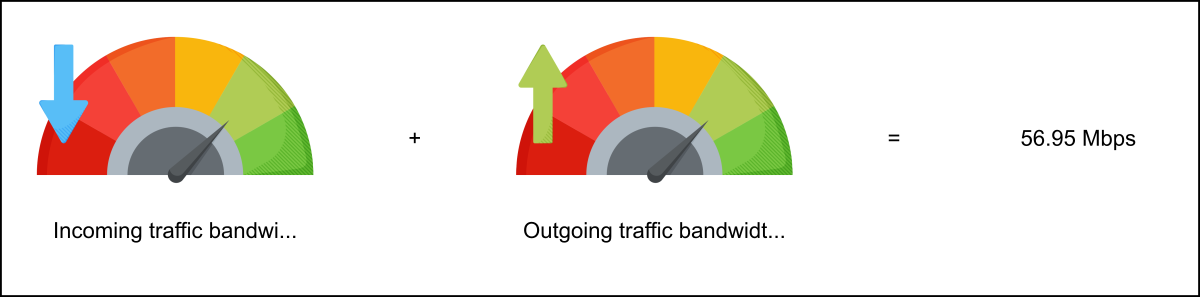
\includegraphics[width=0.5\textwidth]{Images/chapter_21/section_5706146547761152/6162660066721792.png}
 \caption{Summarizing the bandwidth requirements of a video search}
\end{figure}

\begin{quote}
\textbf{Note:} The bandwidth requirements are relatively modest because we are assuming text results. Many search services can return small thumbnails and other media to enhance the search page. The bandwidth needs per page are intentionally low so that the service can provide near real-time results to the client.
\end{quote}
\subsection{Building blocks we will use}\label{pPTH8De0zCFhRVRfDPGEF}
\\
We need a distributed storage in our design. Therefore, we can use the \href{https://www.educative.io/courses/grokking-the-system-design-interview/system-design-a-blob-store}{blob store}, a previously discussed building block, to store the data to be indexed and the index itself. We 'll use a generic term, that is, ``distributed storage'' instead of the specific term ``blob store.''

\begin{figure}[htbp]
 \centering
 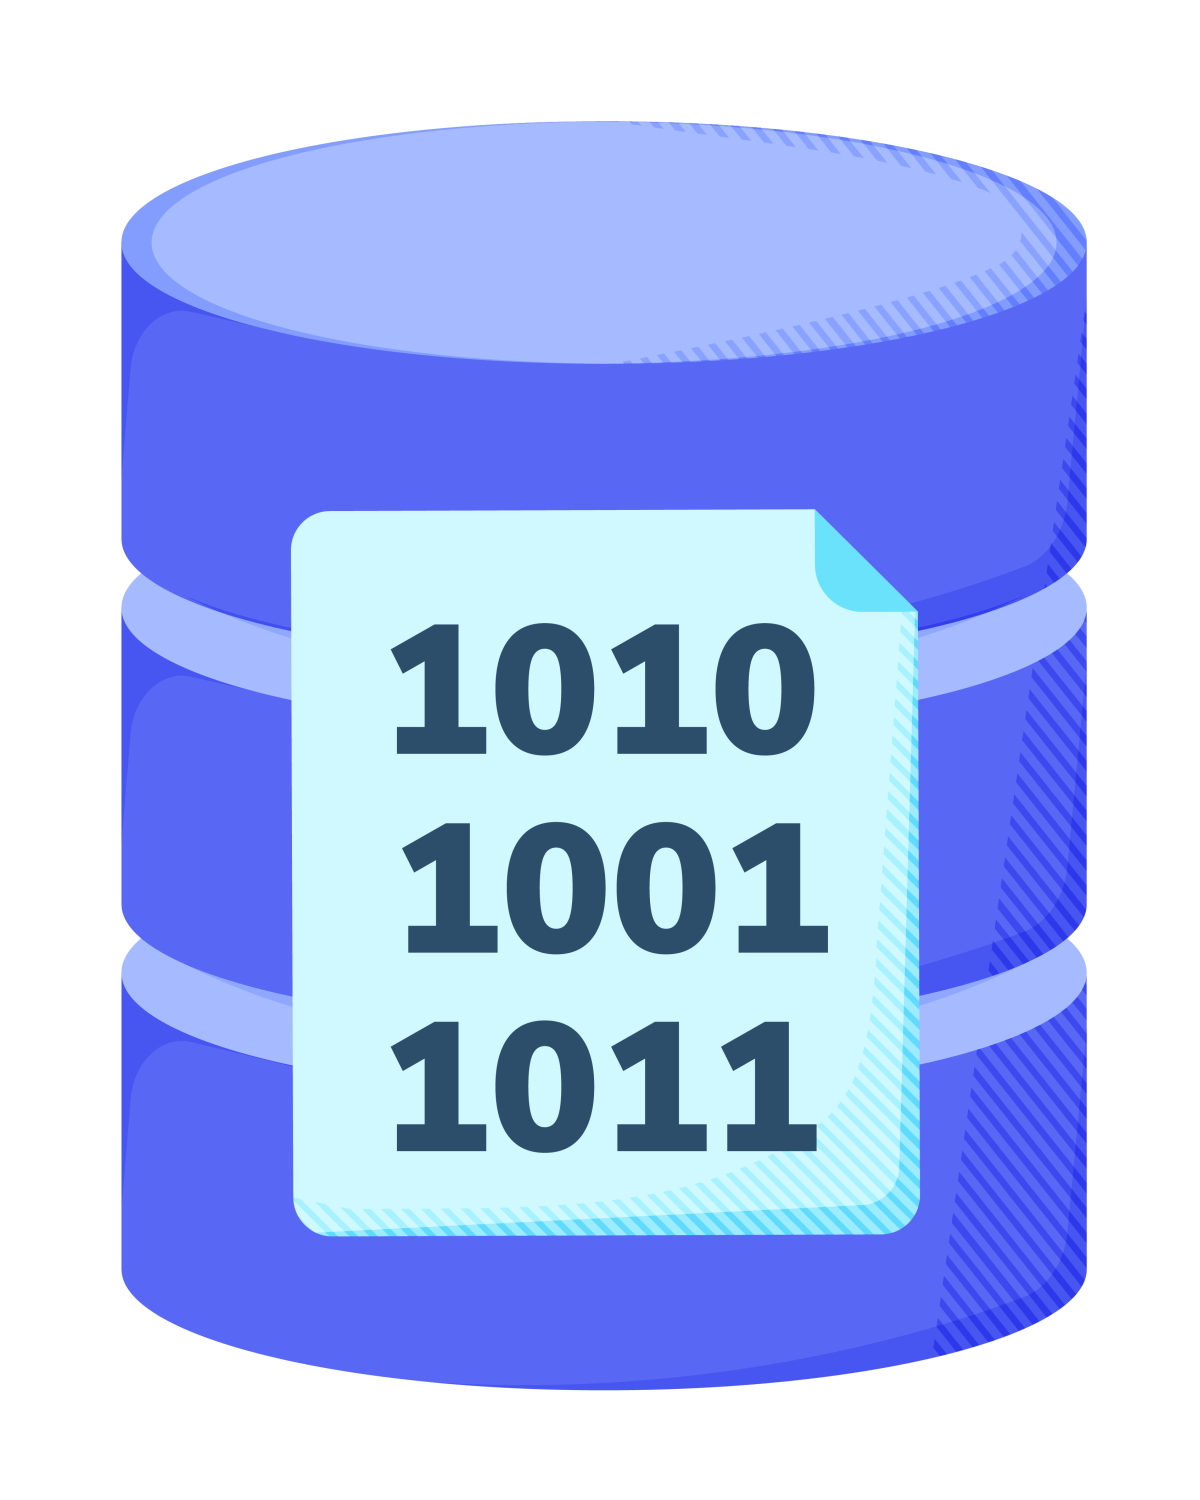
\includegraphics[width=0.15\textwidth]{Images/chapter_21/section_5706146547761152/5578416668409856.png}
 \caption{Distributed storage: Blob store}
\end{figure}

To conclude, we explained what the search system's requirements are. We made resource estimations. And lastly, we mentioned the building block that we'll use in our design of a distributed search system.

% End of section content